\documentclass[letterpaper]{article}
\usepackage[submission]{../AAAI_AuthorKit27/aaai2027}
\usepackage[hyphens]{url}
\usepackage{graphicx}
\urlstyle{rm}
\def\UrlFont{\rm}
\usepackage{natbib}
\usepackage{caption}
\frenchspacing
\usepackage{amsmath,amssymb,amsthm}
\usepackage{booktabs}

\newtheorem{theorem}{Theorem}
\newtheorem{proposition}[theorem]{Proposition}
\newtheorem{corollary}[theorem]{Corollary}
\newcommand{\E}{\mathbb E}
\newcommand{\R}{\mathcal R}
\newcommand{\cS}{\mathcal S}
\newcommand{\wtO}{\widetilde O}

\title{When More Epochs Stop Helping: Coverage-Limited Scaling Laws for Sparse Replay}
\author{Anonymous Submission}
\affiliations{}

\begin{document}
\maketitle

\begin{abstract}
Repeated passes over a fixed dataset can improve optimization, but they cannot
reveal predictive features absent from the unique examples.  We formalize this
distinction in sparse power-law regression, where feature \(j\) activates with
probability \(p_j\asymp j^{-s}\), has covariance eigenvalue
\(\lambda_j\asymp j^{-a}\), and carries target energy
\(g_j\asymp j^{-b}\).  Under a random-sign teacher prior, every learner
incurs a Bayes---and hence minimax---coverage floor
\(\sum_j g_j(1-p_j)^n\asymp n^{-(b-1)/s}\).
An exactly solvable one-hot replay benchmark then yields the three-frontier law
\[
\R(m,n,K)\asymp
m^{-(b-1)}+(\eta nK)^{-(b-1)/a}+n^{-(b-1)/s}.
\]
Our main result extends coverage-limited reuse to genuinely multi-active data.
We analyze support-certified, example-norm-clipped replay SGD, which trains on
all coactive rows.  Natural singleton rows provide coordinate-wise curvature,
while clipping makes every rank-one update a contraction.  We prove that using
all \(n\) examples reaches the coverage floor after
\(\widetilde O(\eta^{-1}n^{a/s-1})\) epochs, and that a
frontier-matched progressive schedule attains the full law above up to
logarithms.  Sparse simulations confirm the predicted transition, source
exponents, and scaling collapse; a two-term fit explains \(98.1\%\) of the
observed risk variation.  The results give a principled stopping rule for
deciding when another epoch is less valuable than another unique example.
\end{abstract}

\section{Introduction}

Power-law learning curves summarize how performance changes with model size,
data, and compute \cite{hestness2017scaling,kaplan2020scaling,
hoffmann2022training,bahri2024explaining}.  They are especially consequential
when data become scarce: one may continue training by repeating the same
examples, but repeated tokens are eventually less valuable than fresh ones
\cite{muennighoff2023scaling}.  This raises a basic allocation question:
\emph{how many epochs are useful for a dataset of a given size?}

Existing linear-regression theory explains how multi-pass optimization can
learn progressively weaker spectral directions
\cite{lin2024scaling,lin2025reuse,chen2026minibatch,zou2022multipass}.
Other analyses prove that the benefit of repetition eventually plateaus for
strongly convex or Zipfian one-hot models \cite{yan2026larger}.  These results,
however, do not separate two facts that coincide in dense data: a direction
can be difficult because its covariance is small, or impossible because the
fixed dataset never contains it.  The distinction matters for sparse,
long-tailed representations, where many predictive coordinates are rare.
Recent sparse-feature theory identifies unobserved coordinates as a new
bottleneck and connects them to asymmetric double descent
\cite{sous2026asymmetric,belkin2019reconciling,hastie2022surprises}, but studies
training to completion rather than the finite-epoch interaction between unique
data and reuse.

We study this interaction in a model with three independently tunable tails:
feature frequency \(p_j\), covariance \(\lambda_j\), and target energy \(g_j\).
The resulting picture has three rank frontiers,
\[
J_{\rm cap}=m,\qquad
J_{\rm opt}=(\eta nK)^{1/a},\qquad
J_{\rm cov}=n^{1/s}.
\]
Their minimum determines the learned scale.  Our contributions are:

\begin{itemize}
\item We prove a Bayes and minimax unseen-feature lower bound, including its
sharp power-law constant.
\item We derive an exact finite-epoch replay law in a one-hot benchmark and
recover the capacity--optimization--coverage frontier.
\item For genuinely multi-active Bernoulli inputs, we resolve the
noncommuting-update obstacle for a concrete all-row algorithm.  Clipped replay
SGD reaches the coverage floor after
\(K_{\rm sat}=\wtO(\eta^{-1}n^{a/s-1})\) epochs.  A progressive-data corollary
achieves the full three-frontier law up to logarithms.
\item Across \(4{,}285\) risk measurements from \(670\) sparse training runs,
we observe the predicted optimization and coverage slopes, collapse curves
across dataset sizes, and show that clipping prevents a high-coactivation
instability.
\end{itemize}

Conceptually, epochs improve the \emph{optimization frontier}; only new
examples move the \emph{coverage frontier}.  This gives a concrete criterion
for switching resources from reuse to data collection.

\section{Related Work}

\paragraph{Scaling laws.}
Empirical power laws were documented across modalities and later used to
optimize language-model resource allocation
\cite{hestness2017scaling,kaplan2020scaling,hoffmann2022training,
rosenfeld2020constructive}.  Theoretical accounts connect exponents to
intrinsic dimension, kernel spectra, and task alignment
\cite{sharma2022manifold,bahri2024explaining,bordelon2020spectrum,
canatar2021spectral}.  Infinite-dimensional linear regression provides sharp
model--data--compute rates under power-law spectra
\cite{lin2024scaling}; data reuse and mini-batching extend this framework
\cite{lin2025reuse,chen2026minibatch}.  The effective-frontier viewpoint
abstracts learning as progressive coverage of a long tail
\cite{zou2026frontiers}.  We provide a concrete sparse stochastic model in
which coverage and optimization are different random mechanisms.

\paragraph{Repeated data and least-squares SGD.}
Data-constrained language-model experiments find that modest reuse can mimic
fresh data before diminishing returns set in
\cite{muennighoff2023scaling}.  Linear-regression analyses study multi-pass
generalization, effective reuse, and finite-dataset fluctuations
\cite{zou2022multipass,yan2026larger}.  Our one-hot formula is a benchmark in
this line; the main contribution is a multi-active theorem where replay
matrices do not commute.  The proof combines classical least-squares SGD and iterate averaging
\cite{polyak1992acceleration,bach2013non,defossez2015averaged,
dieuleveut2016nonparametric,neu2018averaging,ali2020implicit} with a new
occupancy argument tailored to heavy-tailed sparse features.  Clipping is not
cosmetic: sparse conditional amplitudes can make fixed-step dynamics unstable,
as also observed by \citet{sous2026asymmetric}.

\section{Sparse Power-Law Regression}

For \(j\ge1\), let
\[
X_j=q_jZ_jE_j,\qquad
Z_j\sim{\rm Bernoulli}(p_j),\quad E_j\sim{\rm Rad},
\]
independently over coordinates and examples.  Then
\(\lambda_j=\E X_j^2=p_jq_j^2\).  Labels are noiseless,
\(Y=\langle\theta,X\rangle\), and the predictive energy of coordinate \(j\) is
\(g_j=\lambda_j\theta_j^2\).  We assume
\begin{equation}
\begin{gathered}
p_j\asymp j^{-s},\quad
\lambda_j\asymp j^{-a},\quad
g_j\asymp j^{-b},\\
s>1,\qquad a\ge s,\qquad b>1.
\end{gathered}
\label{eq:powerlaws}
\end{equation}
Because \(s>1\), every example has finite support almost surely; the
associated distinct-feature counts are an infinite-urn occupancy process
\cite{karlin1967central}.  Population excess risk is diagonal for linear predictors:
\[
\R(w)=\E_X[\langle w-\theta,X\rangle^2]
=\sum_j\lambda_j(w_j-\theta_j)^2.
\]
For an arbitrary measurable predictor, we use
\(\R(f)=\E_X[(f(X)-Y)^2]\).

For the lower bound, teacher signs are independent Rademacher variables with
fixed magnitudes \(|\theta_j|\).  Let \(D_n\) contain \(n\) unique examples.

\begin{theorem}[Coverage floor]
\label{thm:coverage}
Under the random-sign prior, every measurable, possibly randomized predictor
satisfies
\[
\E_{\theta,D_n}\R(\widehat f)
\ge
\sum_{j\ge1}g_j(1-p_j)^n
\asymp n^{-(b-1)/s}.
\]
For exact \(p_j=c_pj^{-s}\) and \(g_j=c_gj^{-b}\),
\[
\sum_jg_j(1-p_j)^n
\sim
\frac{c_g}{s}\Gamma\!\left(\frac{b-1}{s}\right)
(c_pn)^{-(b-1)/s}.
\]
\end{theorem}

\paragraph{Proof idea.}
If coordinate \(j\) is absent from every training input, no label depends on
its teacher sign.  Conditional on all observed information, that sign remains
symmetric.  Averaging squared test error over the hidden signs leaves at least
the unseen predictive energy.  The asymptotic follows by splitting at
\(j\asymp n^{1/s}\).  Thus no optimizer or number of epochs can beat the
coverage term.  Since a Bayes lower bound is no larger than the corresponding
minimax risk, the same rate is also a minimax lower bound over deterministic
teacher-sign choices.

\section{Exact Replay Benchmark}

In the one-hot benchmark, an example chooses \(J_i\sim(p_j)\) and
\(X_i=E_iq_{J_i}e_{J_i}\).  A width-\(m\) model is trained from zero for \(K\)
passes with step size \(\eta\).  If
\(C_j\sim{\rm Binomial}(n,p_j)\), coordinate updates commute and give the
following exact finite-sample expression.

\begin{proposition}[Exact one-hot replay]
\label{prop:onehot}
For \(0<\eta q_j^2<1\),
\[
\E_{D_n}\R
=
\sum_{j\le m}g_j
[1-p_j+p_j(1-\eta q_j^2)^{2K}]^n
+\sum_{j>m}g_j.
\]
Consequently,
\begin{equation}
\E\R
\asymp
J_\star^{1-b},\qquad
J_\star=\min\{m,(\eta nK)^{1/a},n^{1/s}\}.
\label{eq:threefrontier}
\end{equation}
Equivalently, the risk is within constants of
\[
m^{-(b-1)}
+(\eta nK)^{-(b-1)/a}
+n^{-(b-1)/s}.
\]
\end{proposition}

The survival probability of direction \(j\) is controlled by
\[
np_j\!\left[1-(1-\eta q_j^2)^{2K}\right]
\asymp
\min\{np_j,\eta nK\lambda_j\}.
\]
The first argument is coverage; the second is optimization.  Balancing them
gives, for a sufficiently wide model,
\begin{equation}
K_{\rm sat}\asymp\eta^{-1}n^{a/s-1}.
\label{eq:ksat}
\end{equation}
Related Zipfian one-hot saturation was analyzed by
\citet{yan2026larger}; Proposition~\ref{prop:onehot} serves as our sharp
benchmark for the multi-active problem.

\section{Coactive Replay SGD}

For \(N\) selected examples, let
\[
\cS_N=\bigcup_{i=1}^N{\rm supp}(X_i),\quad
V_N=|\cS_N|,\quad
A_N=\|\theta_{\cS_N}\|_2^2.
\]
A sparse dictionary stores all observed feature identities when \(V_N\le m\).
This makes the selected problem exactly realizable.

At each update, sample a row uniformly with replacement and use
\begin{equation}
\begin{aligned}
\gamma_i&=\min\left\{\eta,\frac{\rho}{\|X_i\|_2^2}\right\},\\
w_{t+1}&=w_t-\gamma_iX_i(X_i^\top w_t-Y_i).
\end{aligned}
\label{eq:clippedsgd}
\end{equation}
where \(0<\rho\le1\), with \(\rho/\|X_i\|_2^2=+\infty\) for a zero row, followed by the Polyak average
\(\bar w_T=T^{-1}\sum_{t<T}w_t\).
We assume \(\eta\sup_jq_j^2\le\rho\).  The algorithm trains on every sampled
coactive row; it does not apply the singleton filter used in our preliminary
achievability result.

To state the bound, define
\[
\alpha=\frac{a-b+1}{s},\qquad
\beta=\frac{b-1}{s},
\]
and assume the source range
\begin{equation}
a-s+1<b<a+1.
\label{eq:source}
\end{equation}
Then \(0<\alpha<1\) and \(\alpha+\beta=a/s\).

\begin{theorem}[Coactive clipped replay]
\label{thm:coactive}
There is an observable support certificate, failing with probability at most
\(N^{-r}+e^{-cm}\) for any fixed \(r>0\), such that whenever
\(N\le c_mm^s\), certified clipped replay satisfies
\begin{equation}
\begin{aligned}
\E\R(\bar w_T)
\le C\bigg[
&\frac{N^\alpha}{\eta T}
+\{\log(eN)\}^{a/s}N^{-\beta}\\
&+N^{-r}+e^{-cm}
\bigg].
\end{aligned}
\label{eq:coactivebound}
\end{equation}
The expectation is over data and replay indices.  On certificate failure the
certified version returns the zero predictor.
\end{theorem}

\paragraph{Why coactivation does not break the rate.}
The probability that a multi-active example is exactly singleton \(j\) is
\[
\nu_j=p_j\prod_{k\ne j}(1-p_k)\asymp p_j,
\]
because \(\sum_jp_j<\infty\).  With high probability, every
\(j\le J_N\asymp(N/\log N)^{1/s}\) has \(\Omega(Np_j)\) singleton rows.
These rows are not filtered; they merely certify curvature inside the full
empirical objective.

Let \(\delta_t=w_t-\theta_{\cS_N}\).  Clipping ensures
\(\gamma_i\|X_i\|^2\le1\), hence every coactive update contracts:
\[
\|\delta_{t+1}\|^2
\le
\|\delta_t\|^2-\gamma_i(X_i^\top\delta_t)^2.
\]
Averaging over the next row and retaining only the nonnegative singleton
contributions gives
\[
\E_t\|\delta_{t+1}\|^2
\le
\|\delta_t\|^2-c\eta
\sum_{j\le J_N}\lambda_j\delta_{t,j}^2.
\]
Telescoping and averaging yield core risk
\(A_N/(c\eta T)\); Euclidean contraction bounds the represented tail by
\(\lambda_{J_N+1}A_N\).  Finally,
\[
\E A_N\asymp N^\alpha,\quad
\E V_N\asymp N^{1/s},\quad
\E\!\sum_{j\notin\cS_N}g_j\asymp N^{-\beta}.
\]
Combining these occupancy laws proves
Theorem~\ref{thm:coactive}.  Full proofs and sharp constants are in the
supplement.

\begin{corollary}[All-data saturation]
\label{cor:alldata}
With \(N=n\), \(T=nK\), and \(m\gtrsim n^{1/s}\),
\[
\E\R(\bar w_{nK})
\lesssim
\frac{n^{\alpha-1}}{\eta K}
+\{\log(en)\}^{a/s}n^{-\beta}.
\]
Therefore \(K=\wtO(\eta^{-1}n^{a/s-1})\) epochs suffice to reach the
algorithm-independent coverage floor, up to logarithms.
\end{corollary}

\begin{corollary}[Full frontier]
\label{cor:full}
Given \(n,m,T\), select
\[
N_\star\asymp
\min\{n,m^s,(\eta T)^{s/a}\}
\]
unique examples and run certified clipped replay.  Then
\[
\begin{aligned}
\E\R(\bar w_T)
\le\wtO\bigl(
&m^{-(b-1)}
+(\eta T)^{-(b-1)/a}\\
&+n^{-(b-1)/s}
\bigr).
\end{aligned}
\]
\end{corollary}

The progressive subset in Corollary~\ref{cor:full} is a conservative
achievability construction, not a claim that discarding data is optimal.
Empirically, using more unique data at fixed updates consistently helps.

\begin{figure*}[t]
\centering
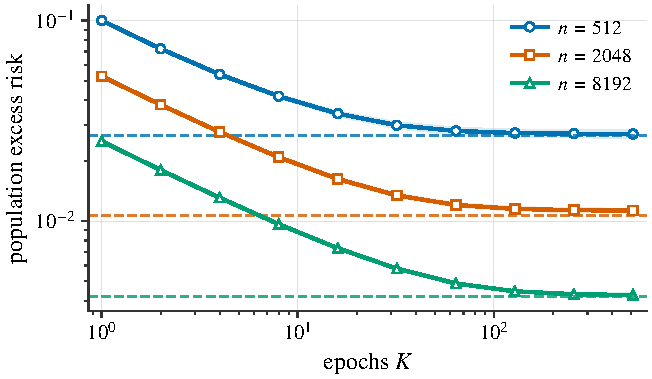
\includegraphics[width=0.485\textwidth]{figures/risk_vs_epochs.pdf}
\hfill
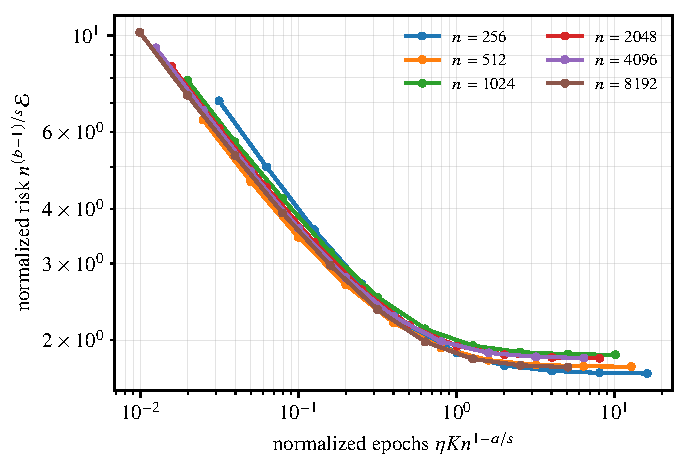
\includegraphics[width=0.485\textwidth]{figures/scaling_collapse.pdf}
\caption{\textbf{Optimization gives way to coverage.}
Left: averaged risk decreases with epochs and plateaus at the independently
computed unseen-feature floor (dashed), whose height moves with the number of
unique examples.  Right: curves collapse after normalizing epochs by
\(\eta n^{1-a/s}\) and risk by \(n^{(b-1)/s}\).  Default
\((s,a,b)=(1.5,2,2)\); means over five seeds.}
\label{fig:main}
\end{figure*}

\section{Experiments}

We generate independent Bernoulli masks directly in sparse CSR form.  Unless
noted otherwise,
\[
p_j=\frac{\mu}{\zeta(s)}j^{-s},\quad
\lambda_j=j^{-a},\quad g_j=j^{-b},
\]
with \((s,a,b)=(1.5,2,2)\), expected active features \(\mu=1\),
\(\eta=0.2\), and ambient dimension \(d=4096\) or \(8192\).  We add the
analytic population tail beyond \(d\).  The primary protocol is
with-replacement clipped replay with \(\rho=0.9\); all main sweeps use five
seeds.  Code computes population risk exactly from the coefficient error.

\paragraph{Three-frontier transition.}
Figure~\ref{fig:main} shows the optimization-limited decay followed by a
unique-data floor.  At \(n=8192\), the early averaged-risk slope is
\(-0.459\), close to the predicted \(-(b-1)/a=-0.5\).  At \(K=512\), the
slope across dataset sizes is \(-0.6548\), versus the predicted
\(-(b-1)/s=-0.6667\).  Fitting all 60 averaged-risk points to
\[
A(\eta nK)^{-(b-1)/a}+Bn^{-(b-1)/s}
\]
gives \(R^2=0.981\) and median relative error \(9.5\%\), without fitting either
exponent.

\paragraph{Progressive compute scaling.}
For total updates \(T\in[2^{12},2^{20}]\), we choose
\(N=\lfloor(\eta T)^{s/a}\rfloor\), as in
Corollary~\ref{cor:full}.  Figure~\ref{fig:progressive} gives slopes
\(-0.502\) for the averaged iterate and \(-0.497\) for the last iterate,
matching \(T^{-(b-1)/a}=T^{-1/2}\).

\begin{figure}[t]
\centering
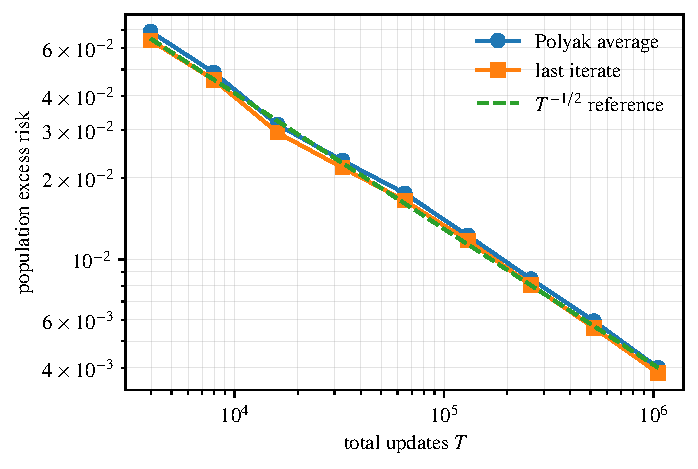
\includegraphics[width=\columnwidth]{figures/progressive_schedule.pdf}
\caption{\textbf{Frontier-matched schedule.}
Choosing \(N\asymp(\eta T)^{s/a}\) yields the predicted
\(T^{-(b-1)/a}=T^{-1/2}\) compute law.}
\label{fig:progressive}
\end{figure}

\paragraph{Source exponents.}
We vary \(b\) while holding \((a,s)=(2,1.5)\).  Table~\ref{tab:source}
shows that the large-epoch data slope tracks \(-(b-1)/s\), including targets
rougher and smoother than the default.  The roughest case \(b=1.4\) lies just
outside the Euclidean-source condition in Eq.~\eqref{eq:source} and is therefore
an empirical robustness test.

\begin{table}[t]
\centering
\caption{Predicted and measured coverage slopes.}
\label{tab:source}
\begin{tabular}{ccc}
\toprule
\(b\) & predicted & measured \\
\midrule
1.4 & -0.267 & -0.263 \\
1.7 & -0.467 & -0.458 \\
2.0 & -0.667 & -0.653 \\
2.4 & -0.933 & -0.915 \\
\bottomrule
\end{tabular}
\end{table}

\paragraph{Unique data at fixed compute.}
At \(T=2^{18}\) updates, increasing unique examples from \(256\) to
\(32{,}768\) reduces last-iterate risk by a factor of \(12.8\), despite
holding total sample updates fixed.  This directly falsifies any law depending
on \(nK\) alone once coverage is active.

\paragraph{Why clipping matters.}
Across expected coactivation \(\mu\in[0.35,2.35]\), clipped cyclic,
reshuffled, and with-replacement replay all approach the same floor.  Under
the aggressive setting \((\mu,\eta)=(2.25,1.2)\), however, unclipped
reshuffling reaches mean risk \(1.16\times10^{85}\) by four epochs, while
clipped replay remains stable and reaches \(7.08\times10^{-3}\), near its
\(6.18\times10^{-3}\) coverage floor.  This supports the contraction mechanism
used in Theorem~\ref{thm:coactive}.

\section{Discussion and Limitations}

The central distinction is between \emph{seeing} a rare feature and
\emph{optimizing} its coefficient.  Repetition addresses only the latter.
The predicted stopping epoch depends on the input exponents \(a,s\), not on
the source exponent \(b\); in principle it can be estimated from unlabeled
feature frequencies and second moments.

Our theorem deliberately isolates this mechanism.  It assumes coordinate-
addressable sparse features, noiseless realizable labels on the selected
dictionary, a source range in which the observed Euclidean teacher norm is
integrable, clipping, and Polyak averaging.  The logarithm comes from requiring
simultaneous singleton coverage of a spectral core.  The unguarded last
iterate and random reshuffling follow the same law empirically, but proving
their sharp pre-saturation rate remains open.  Extending the result to noisy
labels, fixed random sketches, and learned nonlinear features is important
future work.

\section{Conclusion}

Sparse data impose a resource that total updates do not measure: unique
feature coverage.  We derived its unavoidable error floor, characterized its
interaction with model capacity and optimization time, and proved that a
stable coactive replay method reaches it at the predicted epoch scale.
The practical implication is simple: repeat data while optimization is the
active frontier; once the coverage frontier is reached, another unique
example is asymptotically more valuable than another epoch.

\bibliography{references}
\bibliographystyle{../AAAI_AuthorKit27/aaai2027}

\end{document}
